\section{Experimentación y análisis}

\subsection{De Nueva York a Oxford}

Dado que existe un paralelísmo geográfico que acompaña a nuestro análisis, decidimos buscar algo para ejemplificarlo de manera visual. Elegimos la herramienta \textit{IP Fingerprints}\footnote{http://www.ipfingerprints.com/} que nos permite graficar, de forma aproximada, la ubicación de las máquinas por las que se pasa en la ruta, dándonos además, sus coordenadas; y con ellas, la posibilidad de ver en el mapa a dónde corresponden las mismas.\\
\\
\indent Sabemos que de \textit{Nueva York} a \textit{Oxford} hay un cambio de continente en el medio, y eso equivale a \textit{al menos un pasaje por un enlace submarino}. Como vista general, la ruta aproximada es la siguiente:
\begin{center}
	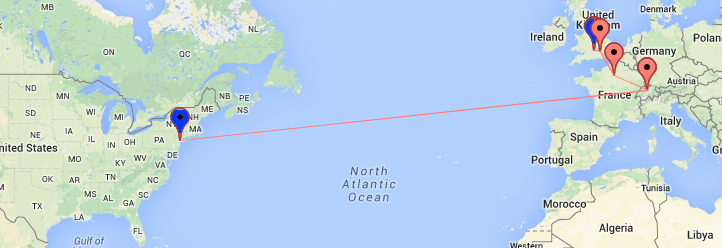
\includegraphics[scale=0.6]{graphics/new_york-oxford.png}
\end{center}

Tal y como lo sospechábamos, podemos observar \textit{enlaces internos en Estados Unidos} y \textit{enlaces internos en Europa}, unidos por un gran \textit{enlace submarino} entre ambos continentes. Decidimos distinguir los nodos de comienzo (en Nueva York) y fin de la ruta (en Oxford) pintándolos de color azul.\\
\\
\indent Viendo un poco más en detalle dentro de Nueva York, esta herramienta nos permitió ver que el primer hop es dentro de la ciudad de Nueva York, como vemos en esta imagen aumentada de la zona:

\begin{center}
	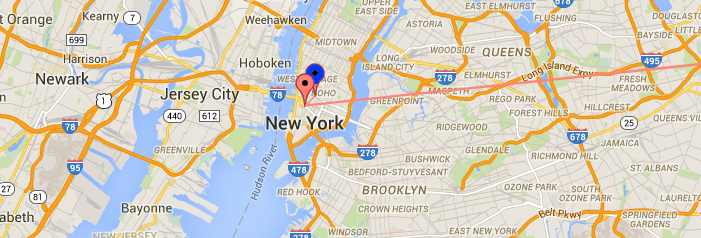
\includegraphics[scale=0.6]{graphics/new_york_zoom.png}
\end{center}

Una vez que sale de ahí, viaja por enlace submarino a Europa. Más precisamente, a Suiza, como se ve en la siguiente imagen aumentada de la zona:

\begin{center}
	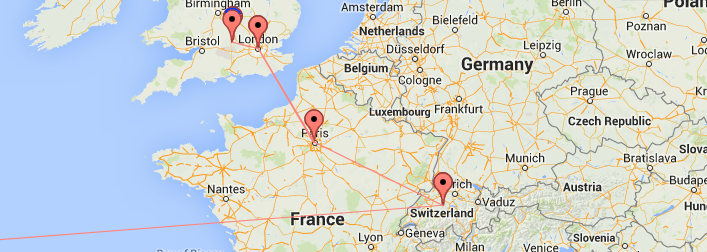
\includegraphics[scale=0.6]{graphics/europe_zoom.png}
\end{center}

Ahí envía paquetes en el mismo país unas 4 veces, hasta que sale y va a Francia, donde se envían 2 paquetes dentro de ese mismo país. Finalmente, de ahí pasa a la isla del Reino Unido, como vemos en la siguiente imagen:

\begin{center}
	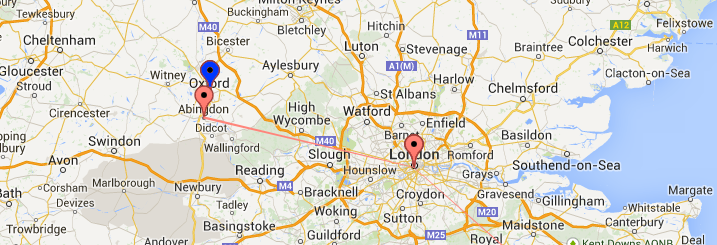
\includegraphics[scale=0.6]{graphics/united_kingdom_zoom.png}
\end{center}

Llega a Lóndres, envía 4 paquetes dentro de la ciudad, para luego ir a la ciudad donde finaliza el camino: Oxford. Ahí llega a la Universidad de Oxford, que es nuestro objetivo, salta a través de 3 máquinas, hasta efectivamente llegar a la que hostea el sitio web de la universidad.

\clearpage

\subsection{De Nueva York a Tokyo}

Empezaremos este análisis revisando la fórmula para \textit{$ZRTT_i$}.

$$ ZRTT_i = \frac{RTT_i - \overline{RTT}}{SRTT} $$

Lo que vemos es que el \textit{z score} de un hop corresponde a la comparación (diferencia) entre su \textit{$RTT_i$} y el RTT promedio, ponderado por el desvío estándar.

Para entender un poco mejor el \textit{z score} veamos qué significa que éste valga 0

\begin{equation}
	\frac{RTT_i - \overline{RTT}}{SRTT} = 0
\end{equation}
\\
\begin{equation}
	\frac{RTT_i}{SRTT} - \frac{\overline{RTT}}{SRTT} = 0
\end{equation}
\\
\begin{equation}
	RTT_i - \overline{RTT} = 0
\end{equation}
\\
\begin{equation}
	RTT_i = \overline{RTT}
\end{equation}

Sabiendo esto, podemos deducir cómo será el \textit{z score} cuando el \textit{$RTT_i$} es mayor al promedio

\begin{equation}
	RTT_i \geq \overline{RTT}
\end{equation}
\\
\begin{equation}
	RTT_i - \overline{RTT} \geq 0
\end{equation}
\\
\begin{equation}
	\frac{RTT_i}{SRTT} - \frac{\overline{RTT}}{SRTT} \geq 0
\end{equation}
\\
\begin{equation}
	\frac{RTT_i - \overline{RTT}}{SRTT} \geq 0
\end{equation}
\\
\begin{equation}
	ZRTT_i \geq 0
\end{equation}

Esto refuerza la intuición de que un RTT mayor al promedio significa un \textit{z score} mayor. Lo que queremos verificar es que a partir de cierto valor de \textit{z score} podemos verificar que se trata un salto transatlántico.

\clearpage

En el caso presentado a continuación presentamos una de varias ejecuciones de nuestro algoritmo desde una instancia del Cloud de Digital Ocean hasta la universidad de Tokyo (www.u-tokyo.ac.jp).

\begin{table}[h]
	\begin{tabular}{l|l|l}
		Z Score & IP & País \\ \hline
		0.964 & 104.131.0.254 & Estados Unidos \\
		-0.599 & 162.243.188.241 & Estados Unidos \\
		0.09 & 62.115.45.9 & Reino Unido \\
		-0.509 & 80.91.248.173 & Francia \\
		-0.327 & 213.155.135.79 & Reino Unido \\
		-0.265 & 129.250.8.29 & Estados Unidos \\
		-0.628 & 129.250.4.172 & Estados Unidos \\
		1.763 & 129.250.2.51 & Estados Unidos \\
		-0.734 & 129.250.2.53 & Estados Unidos \\
		2.755 & 129.250.6.213 & Estados Unidos \\
		-0.274 & 61.213.162.170 & Japón \\
		-0.9 & 61.120.145.170 & Japón \\
		-0.706 & 59.106.85.27 & Japón \\
		-0.152 & 59.106.161.2 & Japón \\
		-0.479 & 59.106.161.29 & Japón
	\end{tabular}
\end{table}

Vemos que valores mayores de \textit{z score} no se condicen necesariamente con saltos entre continentes, pero en el caso donde el valor es 1.763 dentro de Estados Unidos lo notamos en cada una de las ejecuciones del traceroute. Lo mismo para el otro valor que resalta, de 2.755.

Creemos que esto es representativo del ruteo que se da al volver de Europa antes de ir a Japón, donde todos ellos superan valores de \textit{z score} mayores a 1.5, nuevamente, en las diferentes ejecuciones.

\subsection{Universidad de Auckland: de Nueva York a Auckland}


\indent \indent El tercer caso de estudio fue la Universidad de Auckland, ubicada en Nueva Zelanda. Se realizaron diversas corridas del traceroute implementado en distintos horarios del día para obtener así datos más representativos. Una de las primeras cosas que notamos, y que nos llamó la atención fue que en general se seguía una ruta similar independientemente de los horarios del día, contradiciendo la intuición que indicaba que a momentos de mayor carga o congestión la ruta podía variar.\\
\indent Antes de experimentar, habíamos conjeturado que la ruta que más se tomaba debía pasar, en orden, por los Estados Unidos, por Eurasia y finalmente por Oceanía donde llegaba a destino en Nueva Zelanda. A la hora de obtener las localizaciones geógraficas de las direcciones IPs que obtuvimos, sin embargo, nos encontramos frente a diversos problemas. En primer lugar, que las locaciones que nos devolvía nuestra tool no parecían corresponderse con lo que esperábamos. Por lo tanto, comenzamos a localizar las IPs geográficamente utilizando otros servicios. Descubrimos que dependiendo de a qué plataforma le consultábamos la ubicación de la IP los resultados que obteníamos eran totalmente distintos. Basados en los valores de z score que obtuvimos y por nuestras hipótesis, mostramos los resultados que nos produjo utilizar el servicio \url{http://www.ipligence.com/iplocation} que nos permitió ubicar todas las IPs simultáneamente y que se ajustaba a lo que esperábamos para una de las corridas, aunque todos los resultados fueron de la misma forma.\\

\begin{verbatim}
IP                      Continente              País                Región          Ciudad

104.131.0.254           Norteamérica            Estados Unidos      New York        New York 	
162.243.188.229         Norteamérica            Estados Unidos      New York        New York 	
62.115.45.5* 						
80.239.147.139* 						
80.91.254.38* 						
208.173.129.69          Norteamérica            Estados Unidos      Missouri        Chesterfield 	
206.28.99.205           Norteamérica            Estados Unidos      Missouri        Chesterfield 	
206.28.99.70            Norteamérica            Estados Unidos      Missouri        Chesterfield 	
206.28.96.194           Norteamérica            Estados Unidos      Missouri        Chesterfield 	
206.28.97.246           Norteamérica            Estados Unidos      Missouri        Chesterfield 	
208.173.53.142          Norteamérica            Estados Unidos      Missouri        Chesterfield 	
202.84.251.233          Asia                    Hong Kong           Wanchai 	
202.84.142.105          Asia                    Hong Kong           Wanchai 	
134.159.174.42          Asia                    Taiwán 			
203.167.201.42          Oceanía                 Nueva Zelanda       Nueva Zelanda   Auckland 	
130.216.159.127         Oceanía                 Nueva Zelanda       Nueva Zelanda 		

\end{verbatim}


\indent Las direcciones IPs marcadas con un asteriscos son las que más problemas para ubicar nos causaron. Dependiendo del servicio que utilizábamos las direcciones se correspondían a Europa o a los Estados Unidos. Siguiendo nuestras hipótesis y los resultados que obtuvimos, nosotros consideramos que dichas IPs se ubican en los Estados Unidos.\\


\indent Como dijimos anteriormente, una de las particularidades de las corridas que hicimos para este caso de estudio fue que los resultados obtenidos en cuanto a la ruta fue que ésta era similar en cada corrida, incluso con la cantidad de saltos. Si bien esto nos resulta sospechoso, aprovechamos esta oportunidad para promediar los $RTT_i$ de cada salto y calcular así su z-score promedio.\\
\indent En general, para cada corrida detectamos dieciséis IPs distintas, implicando eso quince saltos o hops, dieciséis si contamos la salida a nuestro router local.\\
\indent De las experimentaciones extrajimos el siguiente gráfico que representa el valor de z score promedio que obtuvimos para cada número de salto además de algunos valores de umbral para descartar aquelos enlaces que no son submarinos:\\

\begin{center}
	\includegraphics[scale=0.6]{graphics/zcores-auckland.png}
\end{center}


donde los números de hop se corresponderían siguiendo las IPs mostradas anteriormente, de la siguiente manera:\\

\begin{verbatim}
IP Origen          IP Destino             Número de Hop

-                  104.131.0.254          1
104.131.0.254      162.243.188.229        2
162.243.188.229    62.115.45.5            3
62.115.45.5        80.239.147.139         4
80.239.147.139     80.91.254.38           5
80.91.254.38       208.173.129.69         6 
208.173.129.69     206.28.99.205          7
206.28.99.205      206.28.99.70           8
206.28.99.70       206.28.96.194          8
206.28.96.194      206.28.97.246          10
206.28.97.246      208.173.53.142         11 
208.173.53.142     202.84.251.233         12
202.84.251.233     202.84.142.105         13
202.84.142.105     134.159.174.42         14
134.159.174.42     203.167.201.42         15
203.167.201.42     130.216.159.127        16
\end{verbatim}

\indent Es de notar aquí, que si bien esperábamos un elevado z score para el salto de Estados Unidos a Hong Kong y de Hong Kong a Nueva Zelanda (teniendo en cuenta los que mencionamos en casos anteriores de que un z score alto indicaría un enlace submarino), los valores de z scores que contrastan con los demás por su elevado valor se corresponden a un salto entre dos ubicaciones de Estados Unidos y entre dos locaciones en Hong Kong. A primera vista con los valores obtenidos, creímos haber encontrado que los enlaces submarinos correspondían con los hops números 8 y 12. En ese sentido, que haya dos valores de z scores mucho más elevados que los demás nos indicaba de la existencia de dos saltos intercontinentales, que es lo que habíamos supuesto que ocurriría. No fue hasta luego de la verificación con las direcciones IPs que caímos en la cuenta de que los datos no resultaron como esperábamos. Si un alto valor de z scores indicase enlaces submarinos, con un umbral mayor o igual 1.3 podríamos identificarlos por su valor de z score.\\


